\chapter{Flight Data \label{ch:flight_data}}
After having found the set of optimal calibration parameters and applying them to the flight data of \ac{SETH} junior, roll and pitch angles as well as the gondolas heading or orientation can be calculated. How this is done has been described in sec. \ref{sec:meth:determination_heading} on page \pageref{sec:meth:determination_heading}.

The upper plot in fig. \ref{fig:res:flight_heading} presents the pitch angle in red and roll angle in blue plotted against the \ac{FPGA} time. The lower plot presents the gondolas heading against time. The angle of heading is given from 0 to 360 as it is written on a compass with $0^\circ\equiv\mathrm{North}$, $90^\circ\equiv\mathrm{East}$, etc.\\
It can be seen that the gondola's swinging is strongest after launch and during ascent until it calms down at higher altitudes.

\begin{figure}[H]
    \centering
    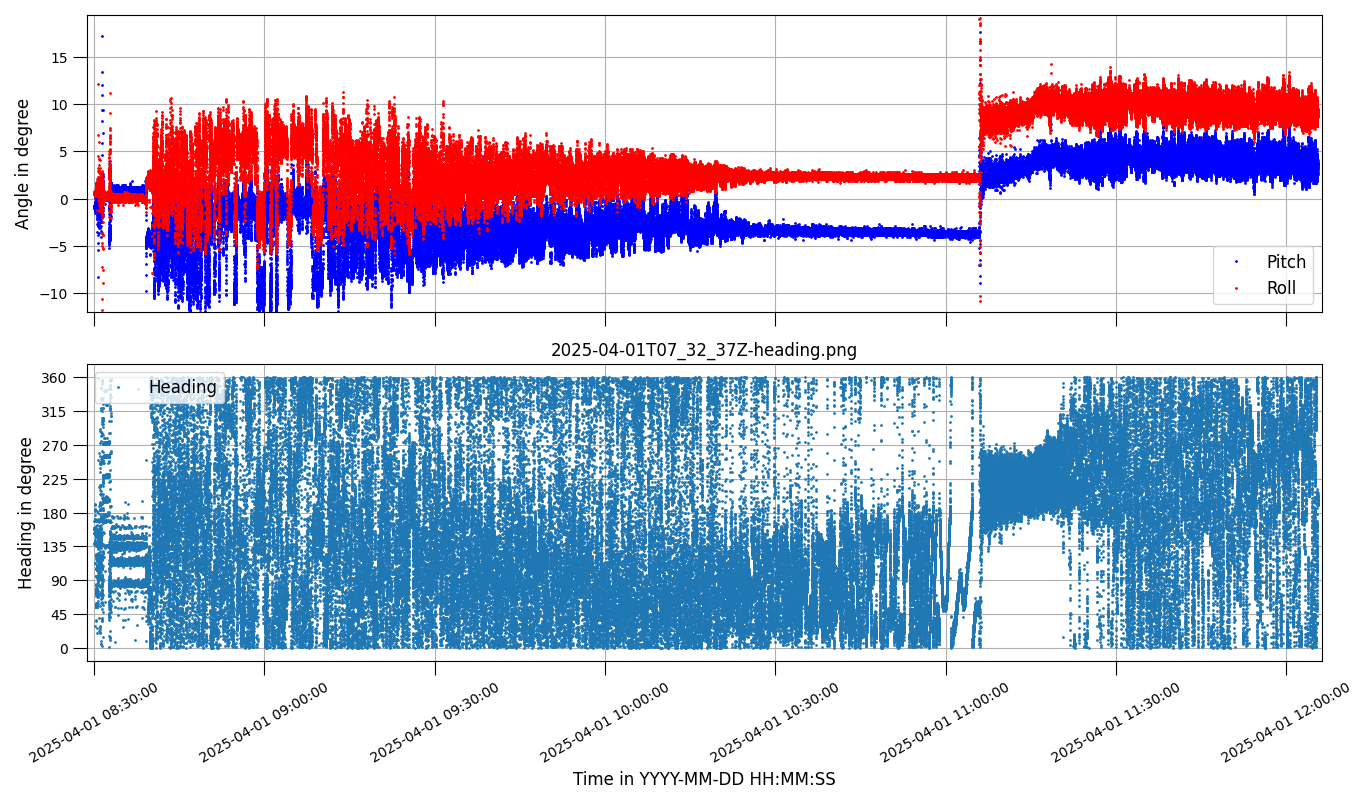
\includegraphics[width=\linewidth]{images/04_results/flight_heading.png}
    \caption{Pitch, roll and heading during the whole flight.}
    \label{fig:res:flight_heading}
\end{figure}

\section{Launch \label{sec:launch}}

\begin{figure}[H]
    \centering
    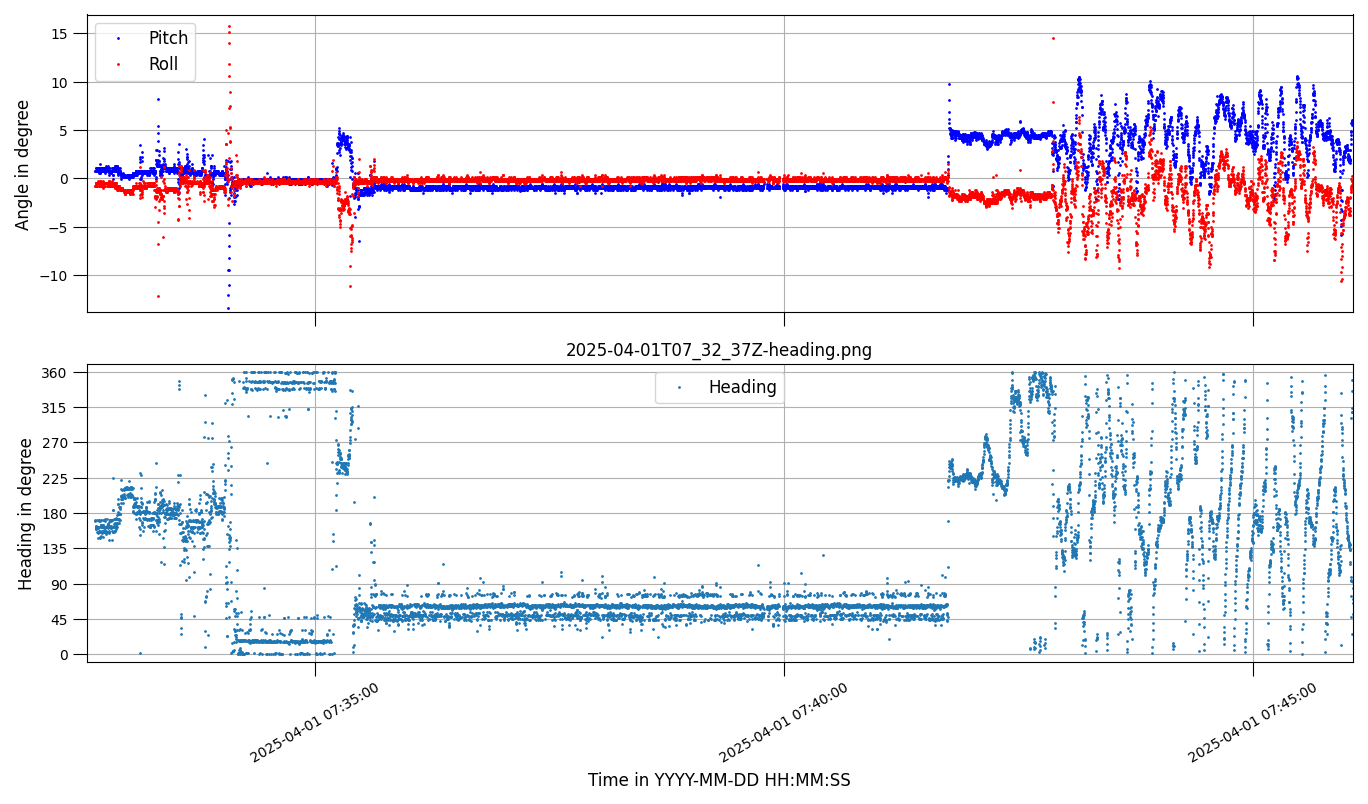
\includegraphics[width=\linewidth]{images/04_results/launch_heading.png}
    \caption[Heading at launch.]{Pitch, roll and heading around launch.}
    \label{fig:res:launch_angles}
\end{figure}


\section{Ascent \label{sec:ascent}}

\begin{figure}[H]
    \centering
    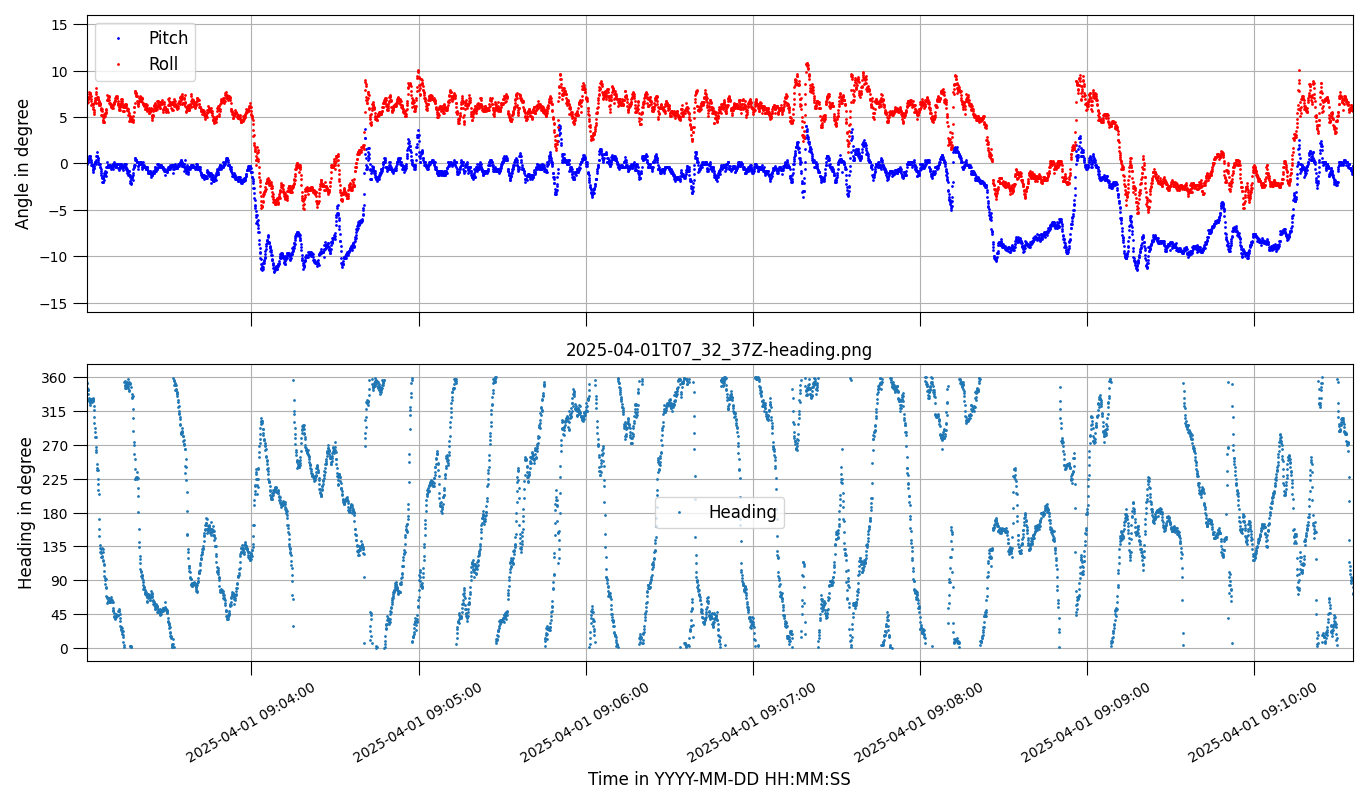
\includegraphics[width=\linewidth]{images/04_results/mid_flight_heading.png}
    \caption[Heading during ascent.]{Pitch, roll and heading during ascent.}
    \label{fig:res:ascent_angles}
\end{figure}


\section{Balloon Burst \label{sec:balloon_burst}}

\begin{figure}[H]
    \centering
    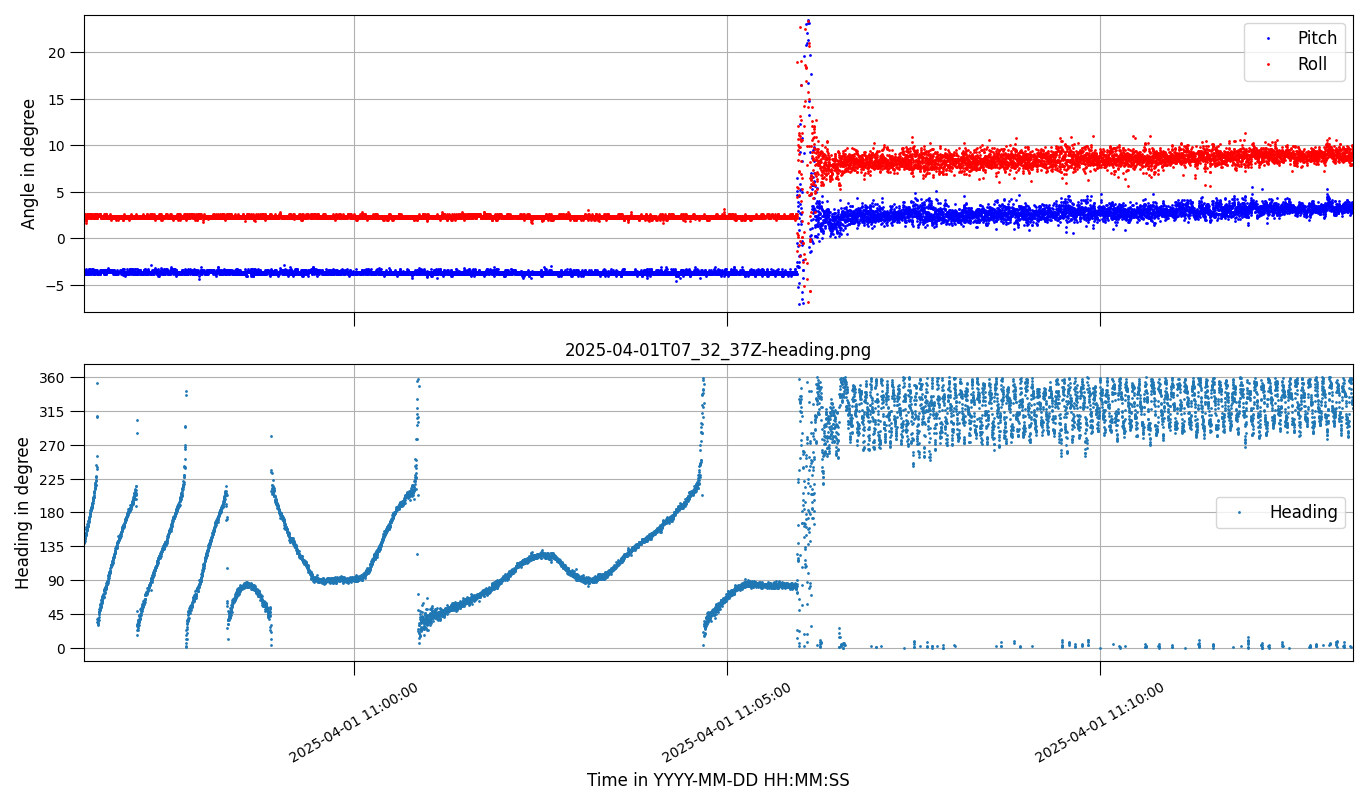
\includegraphics[width=\linewidth]{images/04_results/pop_heading.png}
    \caption[Heading at balloon burst.]{pitch, roll and heading balloon burst.}
    \label{fig:res:pop_angles}
\end{figure}


\section{Descent \label{sec:descent}}

\begin{figure}[H]
    \centering
    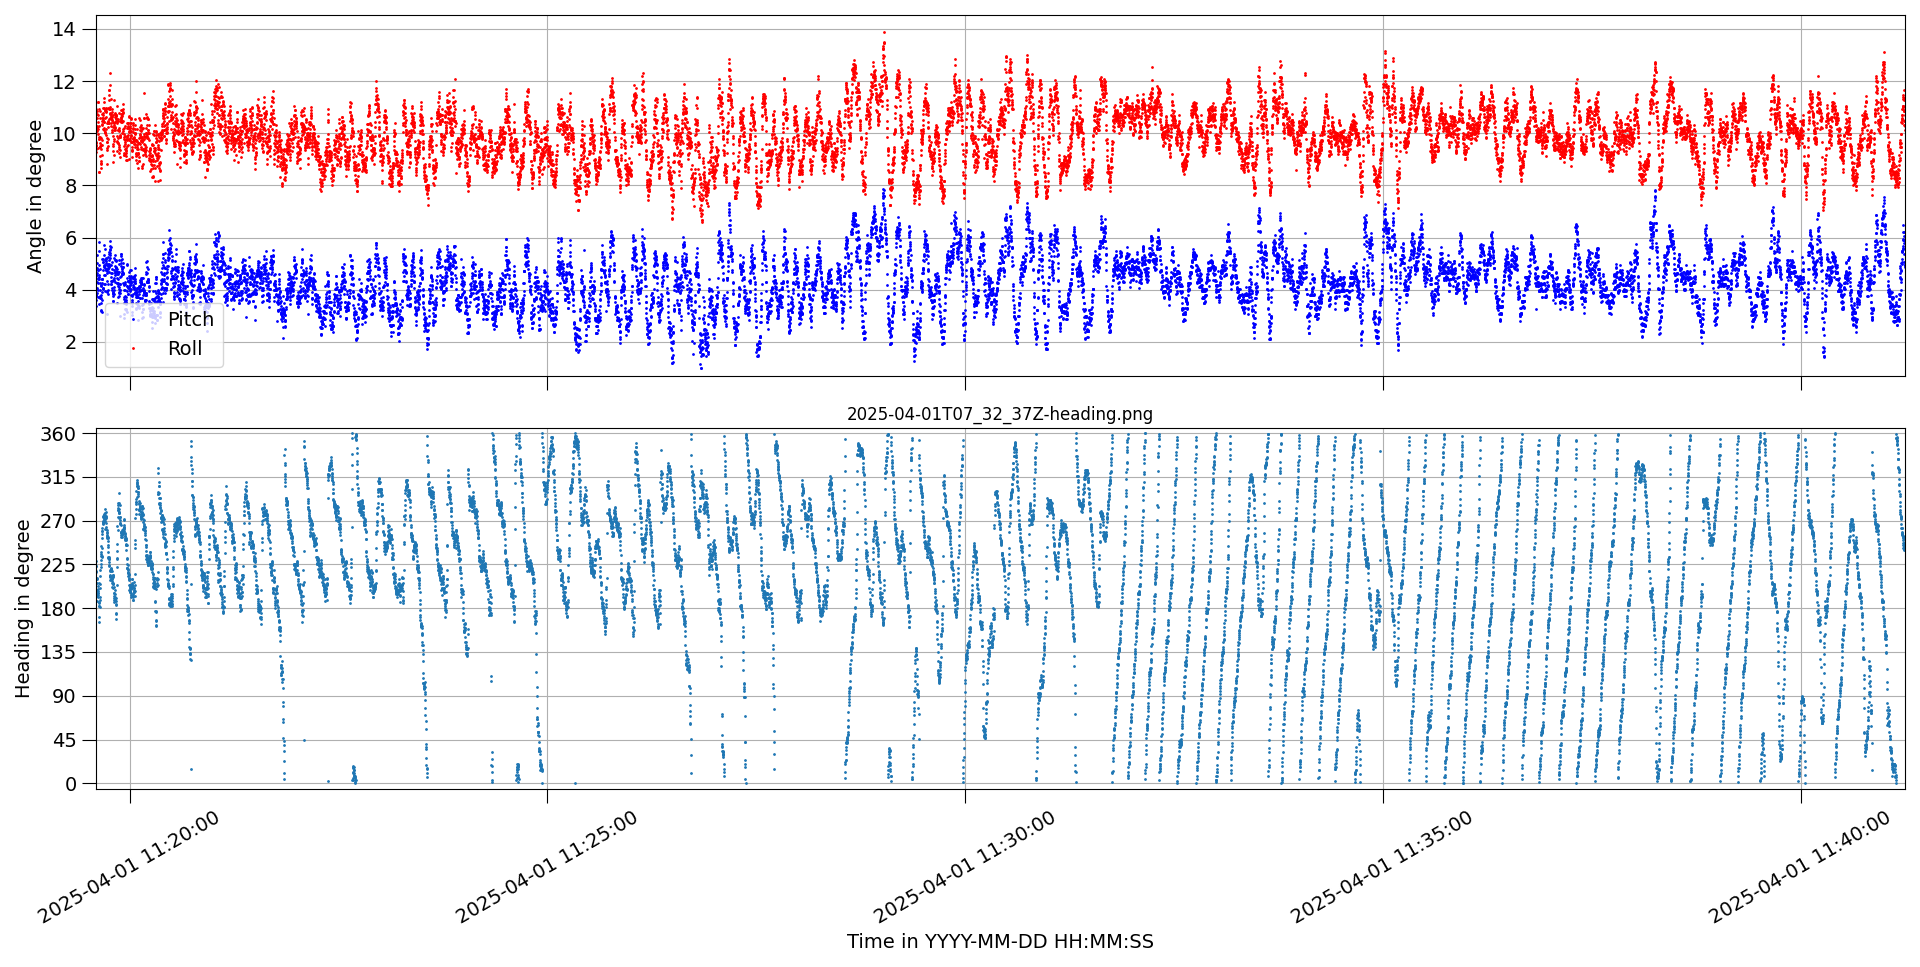
\includegraphics[width=\linewidth]{images/04_results/descend_heading.png}
    \caption[Heading during descent.]{Pitch, roll and heading during descent.}
    \label{fig:res:descent_angles}
\end{figure}